\documentclass[portrait,final,a0paper,fontscale=0.33]{baposter}

%% read in constants, custom functions and used packages

%%%%%%%%%%%%%%%%%%%%%%%%%%%%%%%%%%%%%%%%%%%%%%%%%%%%%%%%%%%%%%%%%%%%%%%% References paths
\usepackage[backend=biber, style=nature, citestyle=nature]{biblatex}
\addbibresource{ActiveSelf.bib}
% font size
\AtBeginBibliography{\scriptsize}

%%%%%%%%%%%%%%%%%%%%%%%%%%%%%%%%%%%%%%%%%%%%%%%%%%%%%%%%%%%%%%%%%%%%%%%% Image paths
\usepackage{graphicx}
\graphicspath{{logos/}{figures/}}

%%%%%%%%%%%%%%%%%%%%%%%%%%%%%%%%%%%%%%%%%%%%%%%%%%%%%%%%%%%%%%%%%%%%%%%% Color Settings
\usepackage{xcolor}
\definecolor{iftucfont}{RGB}{74,130,70}
\definecolor{iftuccolor}{RGB}{143,168,92}
\definecolor{iftucbackground}{RGB}{241,244,234}

%%%%%%%%%%%%%%%%%%%%%%%%%%%%%%%%%%%%%%%%%%%%%%%%%%%%%%%%%%%%%%%%%%%%%%%% Font Settings
\usepackage[sfdefault, regular]{roboto}

%%%%%%%%%%%%%%%%%%%%%%%%%%%%%%%%%%%%%%%%%%%%%%%%%%%%%%%%%%%%%%%%%%%%%%%% Multicol Settings
\usepackage{multirow}
\usepackage{multicol}
\setlength{\columnsep}{1.5em}
\setlength{\columnseprule}{0mm}

%% Row Settings
\usepackage{setspace}% for \onehalfspacing
\usepackage{parskip}

%% Control layout of itemize, enumerate, description
\usepackage{enumitem}

% page borders and header height
\usepackage{geometry}
\geometry{
	left=35pt,
	right=5pt,
	top=10pt
}

\newcommand{\compresslist}{% Define a command to reduce spacing within itemize/enumerate environments, e.g. \begin{itemize}\compresslist
			\setlength{\itemsep}{1pt}
			\setlength{\parskip}{0pt}
			\setlength{\parsep}{0pt}
		}
	
\newcommand{\compressbib}{%
		\setlength{\itemsep}{0pt}
		\setlength{\parskip}{0pt}
		\setlength{\parsep}{0pt}
	}
	
%%%%%%%%%%%%%%%%%%%%%%%%%%%%%%%%%%%%%%%%%%%%%%%%%%%%%%%%%%%%%%%%%%%%%%%% Table and figure settings
\usepackage{float, booktabs, array, ragged2e}

% Adjust row width in tables 
\renewcommand{\arraystretch}{1.1}

% for awesome plots and tables from files like .csv
\usepackage{pgfplots}
\usepackage{pgfplotstable}

% Graphics package-alike macros for “general” boxes. Like resizing figures and aligning minipages
\usepackage{adjustbox}

\usepackage[
font=footnotesize,
labelfont=bf,
%labelfont=sc, %Kapitälchen, passt nicht wg. nicht-osf Ziffern
%%%%labelfont=it, %italics, 
%%%labelfont=sl, %slanted,
hypcap=true,
format=hang,
%margin={2cm,2cm}
width=0.8\linewidth
]{caption}

%%%%%%%%%%%%%%%%%%%%%%%%%%%%%%%%%%%%%%%%%%%%%%%%%%%%%%%%%%%%%%%%%%%%%%%% Other packages
% to help with long equations
\usepackage{amsmath}

% for todo notes
\usepackage{todonotes} 

% for comment blocks
\usepackage{verbatim}

% link URLs
\usepackage{url}

\usepackage{lipsum}


\begin{document}

\begin{poster}%
	% Poster Options
	{
		% Show grid to help with alignment
		grid=false,
		% Number of columns and column spacing
		columns=6,
		colspacing=1em,
		% Color style
		bgColorOne=white,
		borderColor=iftuccolor,
		headerColorOne=iftucbackground,
		headerFontColor=iftucfont,
		boxColorOne=white,
		% Format of textbox
		textborder=rounded,
		textfont=\small,
		% Format of text header
		eyecatcher=true,
		headerborder=closed,
		headerheight=0.1\textheight,
		%  textfont=\sc, An example of changing the text font
		headershape=rounded,
		headershade=plain,
		headerfont=\Large\bf, %Sans Serif
		% textfont={\setlength{\parindent}{1.5em}},
		boxshade=plain,
		%  background=shade-tb,
		background=plain,
		linewidth=2pt
	}
	% University logo
	{\includegraphics[height=6.5em]{tuckhseng_color}} 
	% Title
	{\bf\Large{Developing a body schema by multi-sensory\\ integration through recurrent basis functions and the contribution of the basal ganglia to motor learning}\vspace{5pt}}
	% Authors
	{\large Erik~Syniawa and Fred~Hamker \\ \vspace{0.5em}
	\small Contact: erik.syniawa@informatik.tu-chemnitz.de
	}
	% Department logo and other logos
	{	
		\begin{minipage}[r]{0.1\textwidth}
			
\includegraphics[height=7em]{active_self_logo_color}
		\end{minipage}
		\hfill
		\begin{minipage}[r]{0.1\textwidth}
			
\includegraphics[height=6.5em]{TUC_AI_color}
		\end{minipage}
		
	}

%%%%%%%%%%%%%%%%%%%%%%%%%%%%%%%%%%%%%%%%%%%%%%%%%%%%%%%%%%%%%%%%%%
% use height in headerbox to align multiple boxes 
% height= <size in percent of column height>, else [auto]%
\headerbox{Overview}{name=overview,column=0,row=0, span=3}{
	
	
	\begin{adjustbox}{minipage=0.95\textwidth, margin=5pt, center}

	\begin{minipage}[l]{\textwidth}
		\justifying
		\textbf{Main question:} \\		
		How can a robot develop \textit{awareness} of its own body by associating proprioception with touch and vision using sensory consequences of motor action? \\
		
		\textbf{Neuro-computational model:} \\
		Our model links \textit{sensory representations} within an integrated \textit{body schema}. Predictions and actual sensory results will be considered in the \textit{basal ganglia}. Through cortico-basal ganglia-thalamo (CBGT-) loops the signal transmission will be modulated and dynamically influence the body schema. 
		
		Through \textit{dopamine-modulated plasticity}, the BG enable motor category learning \parencite{segerHowBasalGanglia2008a} and are involved in establishing associations between stimulus and responses \parencite{packardLearningMemoryFunctions2002a}. They act as a kind of reinforcement learning agent.

	\end{minipage}

	\end{adjustbox}
}

\headerbox{\Large Setup}{name=setup,column=3,row=0, span=3}{
	\begin{adjustbox}{minipage=0.95\textwidth, margin=5pt, center}
		\begin{minipage}[l]{0.5\textwidth}
			\vspace{1pt}
			
			\centering
			\includegraphics[width=0.75\linewidth]{robot_setup}
			\captionof{figure}{Current virtual robot setup.}
		\end{minipage}
		\begin{minipage}[l]{0.5\textwidth}
			\textbf{Task:} \\
			Based in 2D-plane a robot should touch this right forearm. He develops the plan and visually fixates the correspondes point on this forearm. 
		\end{minipage}
	\end{adjustbox}
}

\headerbox{\large Computational Model}{name=network, column=0, below=overview, span=3, height=0.45}{
	\begin{adjustbox}{minipage=0.95\textwidth, margin=5pt, center}
	% Network definitions
	\centering
	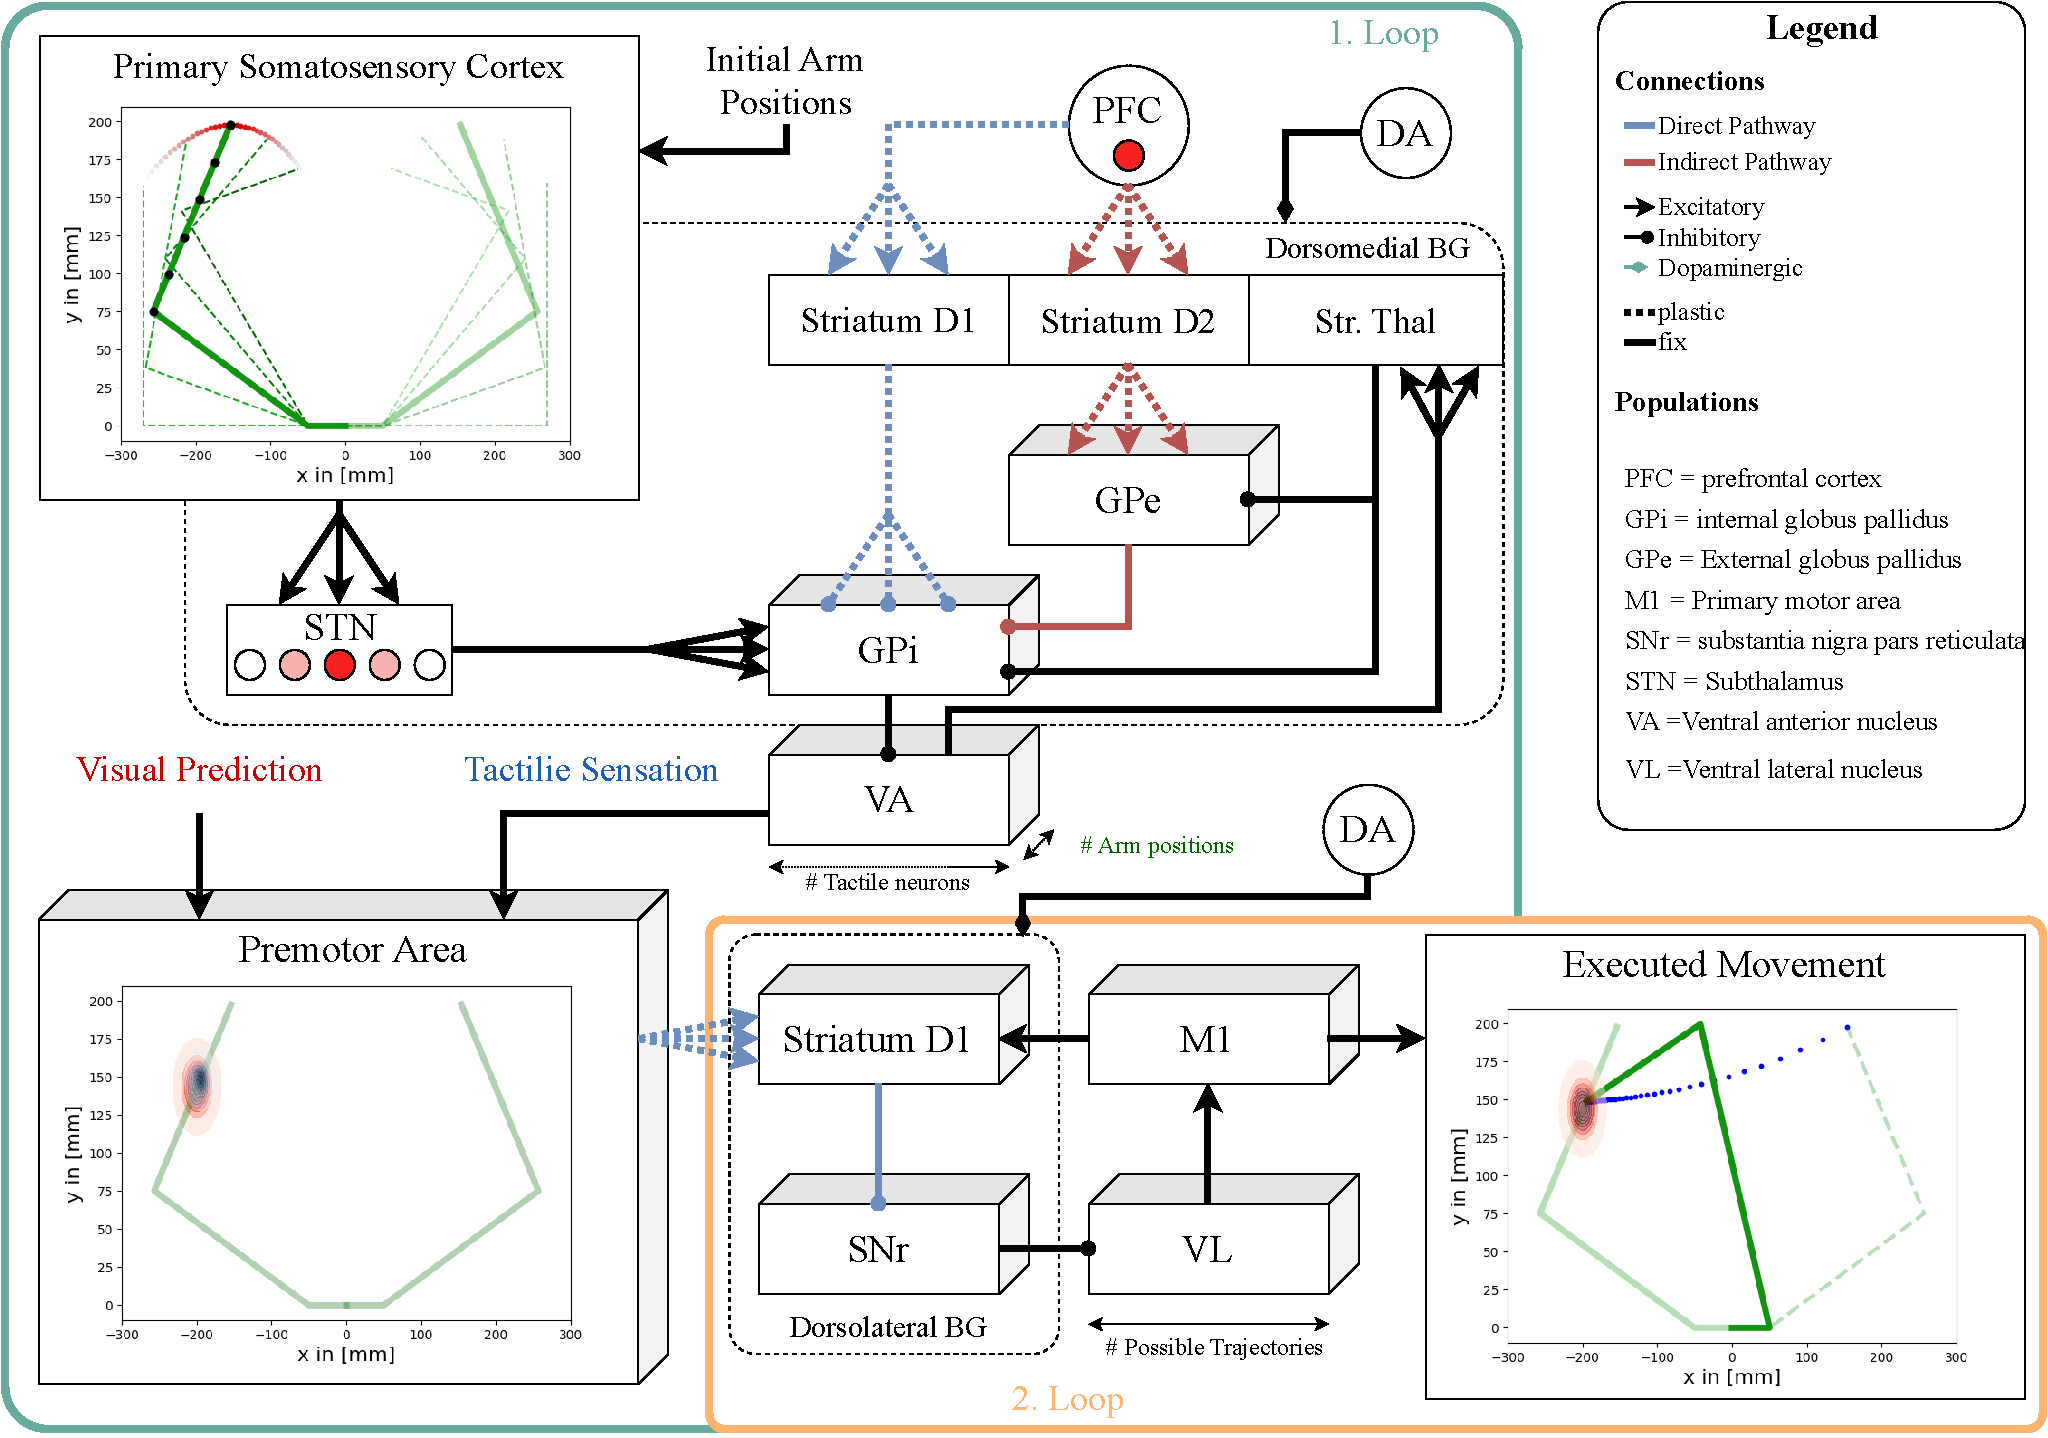
\includegraphics[width=\linewidth]{BG_inverse_model}
	\captionof{figure}{Overview of the whole model.}
	
	\justifying	
	\begin{multicols}{2}
	
	\textbf{Network of the Basal Ganglia (BG):}\\
	
	Our model consist of 2 CBGT-Loops. The first one \ldots

	
	\end{multicols}
	\end{adjustbox}
}

\headerbox{\large Network definitions}{name=plastic, column=3, below=setup, span=3, height=0.405}{
	\begin{adjustbox}{minipage=0.95\textwidth, margin=5pt, center}
		
		\begin{minipage}[l]{0.5\textwidth}
			\textbf{Learning in the different pathways:}\\
			\justifying
			
			The learning principles are primarily determined by \textit{presynaptic} and \textit{postsynaptic} activity, as well as the \textit{Dopamine signal} (\textbf{DA}). Together these principles form a 3-factor learning rule (see Table 1, modified after \cite{maithOptimalAttentionTuning2021c}).
			\vspace{1pt}
			\begin{itemize}
				\item \textit{High} and \textit{low} indicate whether the pre- and post-activity is more than or less than a given threshold (e.g. mean activity).
				\item \textit{DA+} and \textit{DA-} labels indicate if the DA levels exceed a given threshold or not.
			\end{itemize}
			\vspace{10pt}
		\end{minipage}
		\hfill
		\begin{minipage}[r]{0.45\textwidth}
			\begin{itemize}
				\item The sign \textit{+} or \textit{-} represents the weight changes in the relevant projections for each combination.
			\end{itemize}
			\begin{flushright}
				\raggedleft
				\resizebox{\columnwidth}{!}{%
	\begin{tabular}{lcccccl}
		\multicolumn{2}{l}{\multirow{4}{*}{}}          & \multicolumn{4}{c}{\textbf{Dopamine}}               & \multirow{4}{*}{}                    \\ \cline{3-6}
		\multicolumn{2}{l}{}                           & \multicolumn{2}{c}{DA +} & \multicolumn{2}{c}{DA -} &                                      \\ \cline{3-6}
		\multicolumn{2}{l}{}                           & \multicolumn{4}{c}{\textbf{Post-activity}}          &                                      \\ \cline{3-6}
		\multicolumn{2}{l}{}                           & High        & Low        & High        & Low        &                                      \\ \hline
		\multirow{8}{*}{\textbf{Pre-activity}} & High & +           &            & -           &            & \multirow{2}{*}{\textbf{Cortex-D1}}  \\
		& Low  & -           &            &             &            &                                      \\ \cline{2-7} 
		& High & -           &            & +           &            & \multirow{2}{*}{\textbf{Cortex-D2}}  \\
		& Low  &             &            & -           &            &                                      \\ \cline{2-7} 
		& High & -           & +          &             & -          & \multirow{2}{*}{\textbf{D1-GPi}}     \\
		& Low  &             &            &             &            &                                      \\ \cline{2-7} 
		& High &             & -          & -           & +          & \multirow{2}{*}{\textbf{D2-GPe}}     \\
		& Low  &             &            &             &            &                                      \\ \hline
	\end{tabular}
}
				\captionof{table}{Overview 3-factor learning.}
			\end{flushright}
		\end{minipage}
		\textbf{Neuron model:}\\
		\footnotesize
		\textit{All Populations:} 
		$$
		\tau \frac{d r^{post}_i }{ dt } + r^{post} = \sum_{exc}{w \cdot r^{pre}} - \sum_{inh }{w \cdot r^{pre}} + baseline + \xi \hspace{5em} \text{with:  } \xi \sim \mathcal{U}
		$$

		\textbf{Synaptic learning rule:}\\
		$$\tau_w \frac{d w_{ij} }{ dt } = m_{DA} \cdot C_{ij} - \alpha \left(r^{post}_j - \bar{r}^{post} - \gamma^{post}\right)^2 \hspace{5em} \tau^{\alpha} \frac{d \alpha_j }{ dt } + \alpha_j = (r^{post}_j - \Theta)$$ 
		$$
		m_{DA} = const \cdot DA_{type} \left(r^{DA} - baseline_{DA}\right) \hspace{2em} \text{with:  } DA_{type} = \begin{cases} +1 & \text{direct pathway}  \\ -1 & \text{indirect pathway}  \end{cases}
		$$
		
		\textit{Cortico-striatal:}
		$$ C_{ij} = \left(r^{pre}_j - \bar{r}^{pre} - \gamma^{pre}\right)^+ \left(r^{post}_j - \bar{r}^{post} - \gamma^{post}\right) $$
		\textit{Striatal-pallidal:} 
		$$ C_{ij} = \left(r^{pre}_j - \bar{r}^{pre} - \gamma^{pre}\right)^+ \left(\bar{r}^{post} + \gamma^{post} - r^{post}_j \right) $$
	\end{adjustbox}
}

\headerbox{\large References}{name=refs, column=0, above=bottom, span=6}{
	\begin{adjustbox}{minipage=0.98\textwidth, margin=0pt, center}
		
		\compressbib{\printbibliography[heading=none]}

		
	\end{adjustbox}
	
	
}


\headerbox{\large Combining }{name=bg, column=0, below=network, above=refs , span=3}{
	\begin{adjustbox}{minipage=0.95\textwidth, margin=5pt, center}
		
	
		\begin{minipage}[l]{0.45\textwidth}

			
		\end{minipage}
		\hfill
		\begin{minipage}[r]{0.55\textwidth}
			\begin{flushright}
				\raggedleft
				\includegraphics[width=\linewidth]{BG_Learning}
				\captionof{figure}{Weight changes in the 1. BG-Loop}
			\end{flushright}
			
		\end{minipage}
	\end{adjustbox}

}

\headerbox{\large Motor Learning in the Basal Ganglia}{name=motor, column=3, below=plastic, above=refs , span=3}{

	\begin{adjustbox}{minipage=0.95\textwidth, margin=5pt, center}
		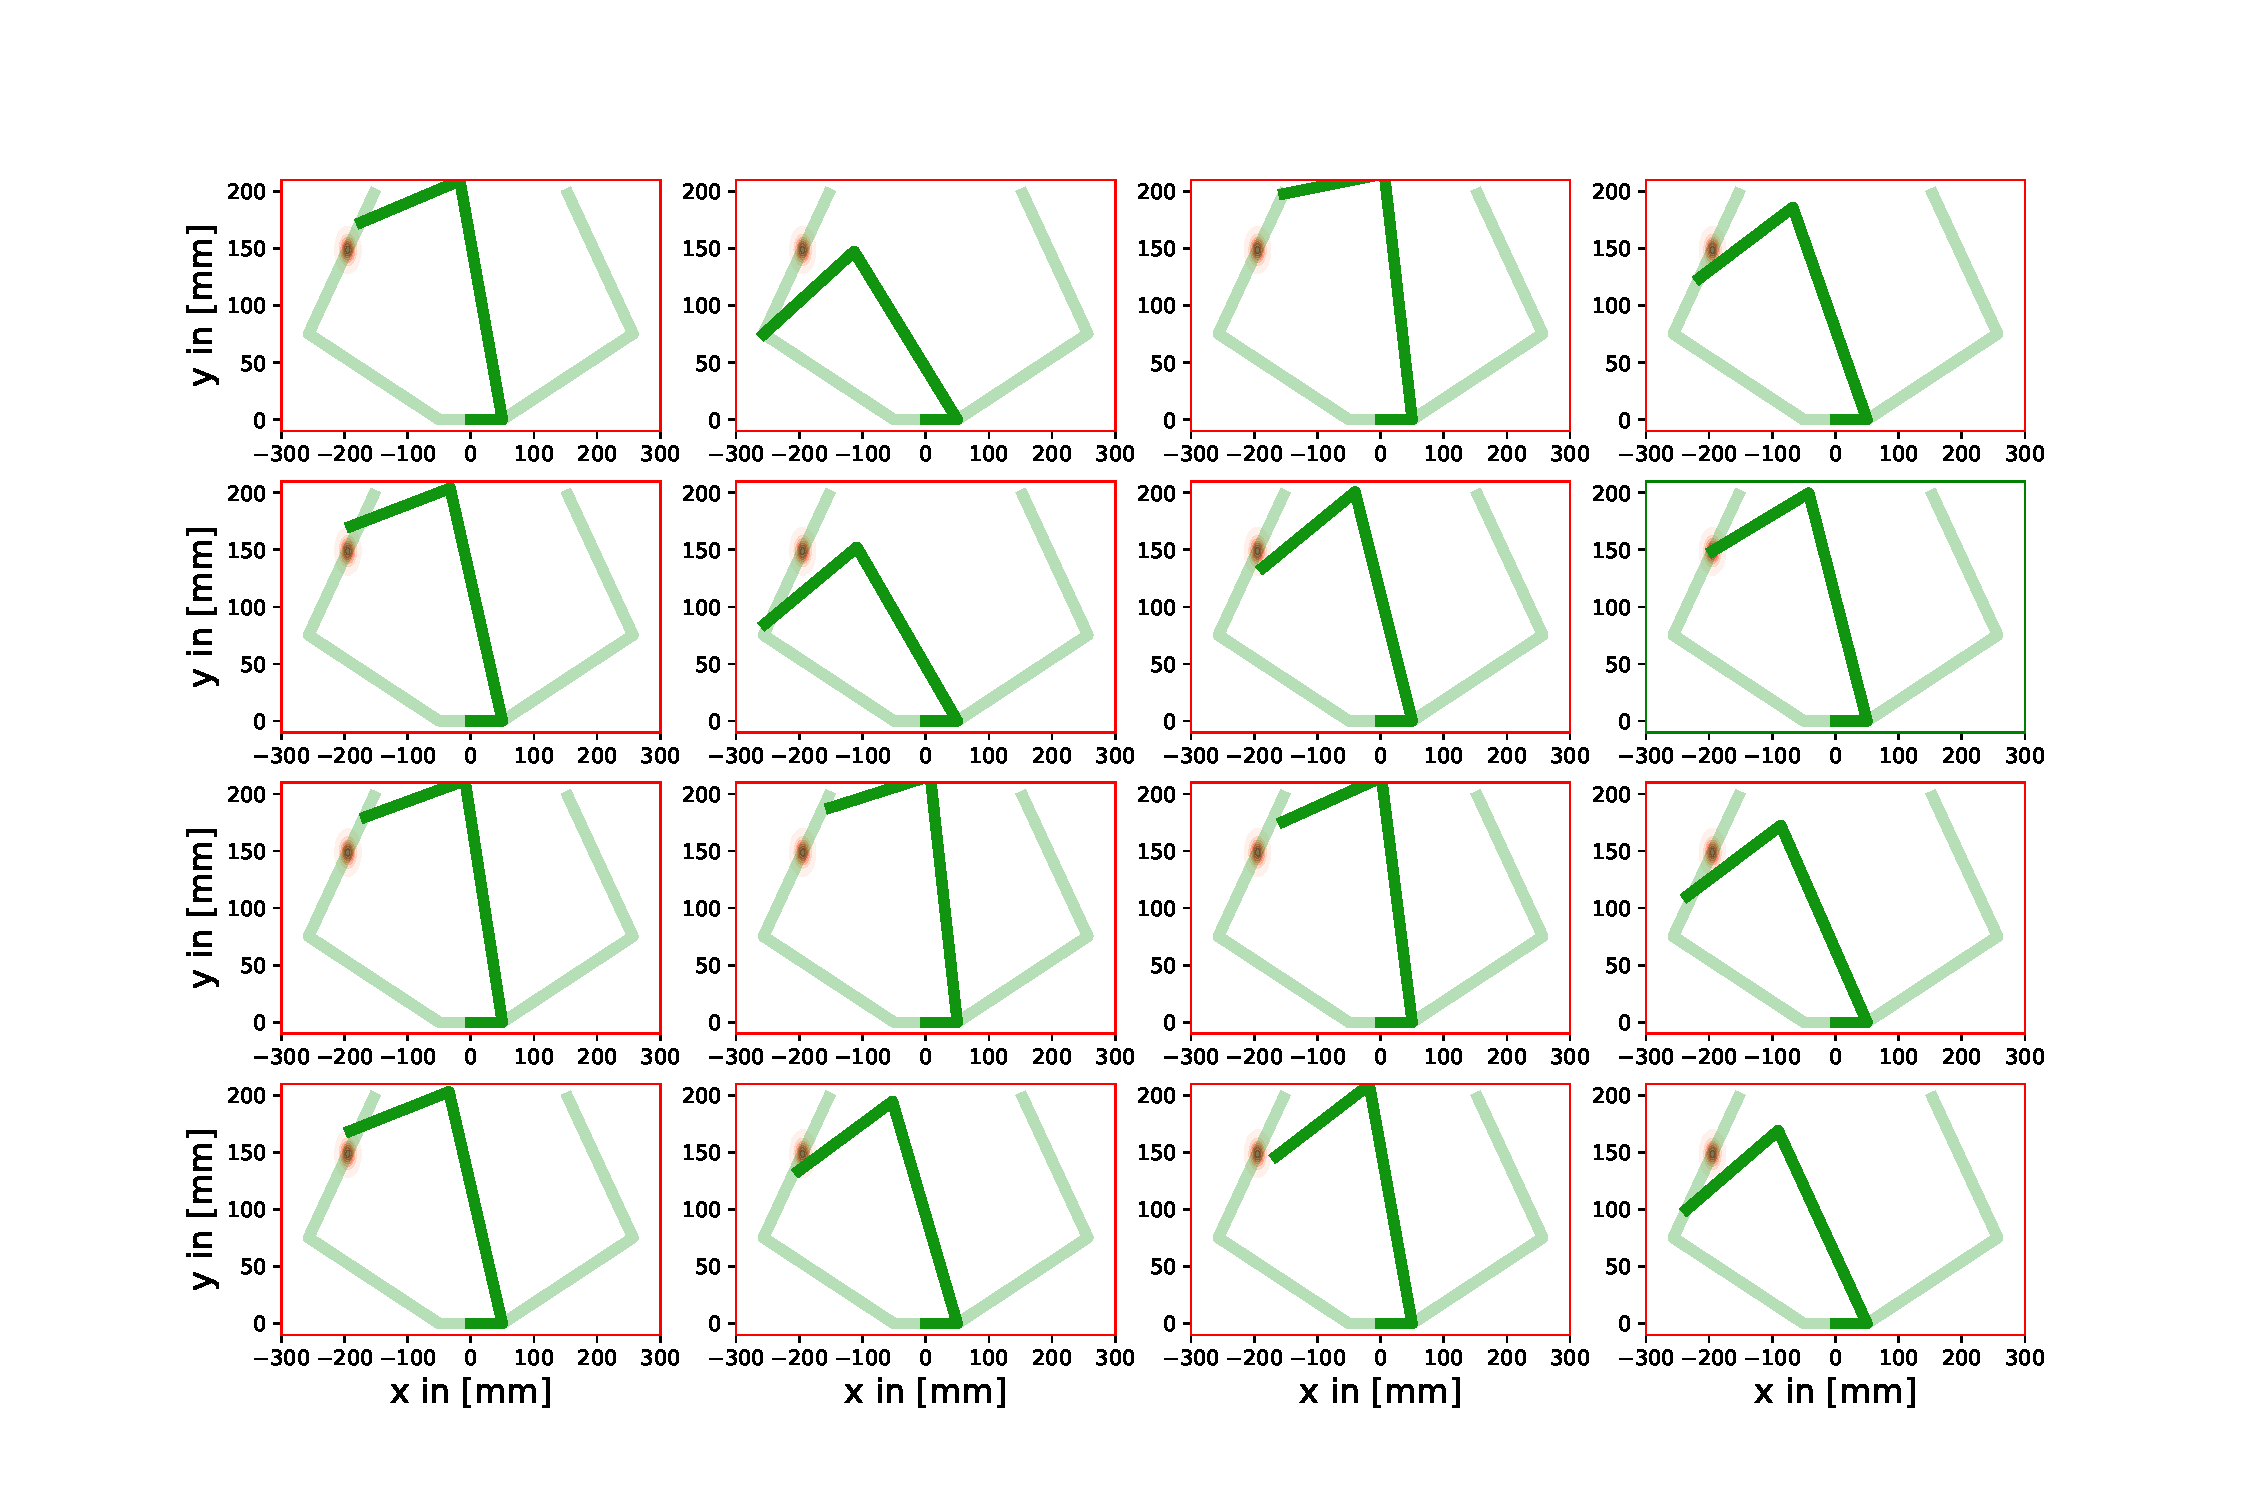
\includegraphics[width=\linewidth]{trajectories}
		\captionof{figure}{Weight changes in the 1. BG-Loop}
		
		\textbf{Learning motor skills through motor babbling:}\\
		
		
	\end{adjustbox}

}


\end{poster}


\end{document}